\section{Microservice Architecture}
\label{se:microservice}

The microservice architectural style is an approach to developing a single application as a suite of small services, each running in its own process and communicating with lightweight mechanisms, often via providing \hl{an RESTful API}. These services are built around business capabilities and independently deployable by fully automated deployment machinery \cite{LewisMicroservices}. \hl{These services are implement independently with minimising the centralized dependencies. Thus each microservice may be written in different programming languages and use different data storage technologies}.

% \hl{Among the characteristics of microservice, a few characteristics heavily affect while moving from} \acrshort{soa} to microservice.
\dbc{M in Microservice should be capitalized only on begining of a sentence.}

There are lots of microservice patterns developed and evolved over the time. Through out the following sections, we will discuss in brief about some of the microservice design patterns mostly used on the context of designing \acrshort{wdias} architecture. Next, we will discuss about how microservice architecture promote to only to create endpoints which are only belongs to each service logical domain. Next discuss about only using database per service which allows to loosely couple between system and achieve high scalability. In Sagas, we discuss about how distributed transaction can achieve over microservices. Next, we will discuss about a concept called as \emph{scale cube}, which explains the scalability in perspective of x,y and z axis.


%%%%%%%%%%%%%%%%%%%%%%%%%%%%%%%%%%%%%%%%%%%%%%%%%%%%%%%%%%%%%%%%%%%%%%%%%%%%%%%%
\subsection{Smart Endpoints and Dumb Pipes}
\label{subse:dumb_pipes}
\dbc{At the end of previous para tell what will be discussed in the next set of sub-section. A single sentence like "Next, we will discusss ...." is enough}
\gkc{FIXED}

When building communication endpoints, \hl{many architectural approaches are adding significant smart by providing different protocol supports and complex logic support via the endpoints.} As an example \acrshort{esb} support multiple protocols and endpoints can use complex logic. But microservice follows alternative approach: \emph{Smart endpoints and dumb pipes} \cite{LewisMicroservicesPipes}.
Applications built from microservices aim to be as decoupled and as cohesive as possible. They own their own domain logic and act more as filters in the classical Unix sense. After receiving a request, applying logic as appropriate and producing a response. And it uses simple RESTful protocols rather than complex protocols.
\dbc{RESTish or RESTful?}
\gkc{Yes. Changed.}

%%%%%%%%%%%%%%%%%%%%%%%%%%%%%%%%%%%%%%%%%%%%%%%%%%%%%%%%%%%%%%%%%%%%%%%%%%%%%%%%
\subsection{\hl{Database per Microservice}}
\label{subse:database_per_service}

\acrshort{microservice} prefer letting each service manages its own database, either different instances of the same database technology, or entirely different database systems - an approach called \emph{Polyglot Persistence} \cite{LewisMicroservicesManagement}.

The idea is to keep each microservice’s persistent data private to that service and accessible only via its \acrshort{api}. 
There are a few different ways to keep a service's persistent data private. It is not need to provision a database server for each service. For example, in the case of using a relational database then following methods can be use to keep data private \cite{RichardsonMicroservicesService}:
\begin{itemize}
    \item \emph{Private tables per service} –- each service owns a set of tables that must only be accessed by that service
    \item \emph{Schema per service} –- each service has a database schema that’s private to that service
    \item \emph{Database server per service} -– each service has its own database server.
\end{itemize}
\emph{Private tables per service} and \emph{schema per service} have the lowest overhead. Using a \emph{schema per service} is appealing since it makes ownership clearer. Some high throughput services might need their own database server.

%%%%%%%%%%%%%%%%%%%%%%%%%%%%%%%%%%%%%%%%%%%%%%%%%%%%%%%%%%%%%%%%%%%%%%%%%%%%%%%%
\subsection{\hl{Distributed Transactions over Microservices}}
\label{subse:sagas}
In order to ensure loose coupling, each microservice better to have own database. Maintaining data consistency between services is a challenge because 2 phase-commit/distributed transactions is not an option for many applications. A service publishes an event when its data changes. Other services consume that event and update their data \cite{RichardsonMicroservicesSagas}. This is also called as \emph{Saga pattern}.

%%%%%%%%%%%%%%%%%%%%%%%%%%%%%%%%%%%%%%%%%%%%%%%%%%%%%%%%%%%%%%%%%%%%%%%%%%%%%%%%
\subsection{\hl{Concept of Scale Cube}}
\label{subse:scale_cube}
\gkc{I can not think about any other title than this.}
The scalability of a system can explain via a concept called \emph{Scale Cube} which talk about the scalability of the application by defining over X, Y and Z axis.

\paragraph{X-axis Scaling}-- X-axis scaling consists of running multiple copies of an application behind a load balancer. If there are \textit{n} copies then each copy handles 1/\textit{n} of the load. This is a simple, commonly used approach of scaling a service.

\paragraph{Y-axis Scaling}-- Unlike X-axis and Z-axis, which consist of running multiple, identical copies of the application, Y-axis axis scaling splits the application into multiple, different services. Each service is responsible for one or more closely related functions. There are a couple of different ways of decomposing the application into services.
\begin{itemize}
    \item verb-based decomposition e.g., checkout.
    \item decompose the application by noun, for e.g., customer management. 
    \item an application might use a combination of verb-based and noun-based decomposition.
\end{itemize}

\emph{The microservice architecture is an application of Y-axis scaling}.

\paragraph{Z-axis Scaling}-- When using Z-axis scaling each server runs an identical copy of the code (similar to X-axis scaling). The big difference is that each server is responsible for only a subset of the data. 
Z-axis splits are commonly used to scale databases. Data is partitioned (a.k.a. sharded) across a set of servers based on an attribute of each record.

Even \acrshort{wdias} is design based on the Y-axis scaling, it's possible to use the Z-axis scaling to scalability of the system further. This will be more discuss in the \cref{se:discussion}.


%%%%%%%%%%%%%%%%%%%%%%%%%%%%%%%%%%%%%%%%%%%%%%%%%%%%%%%%%%%%%%%%%%%%%%%%%%%%%%%%
% \subsection{Brief introduction to the \acrfull{k8s}}
% \label{sebse:k8s_intro}
\dbc{Don't present this as a separate section. Either this need to be in the literature survey, or integrate key ideas into another section as a paragraph.}
\gkc{Move this as a paragraph at the end of the architectural decisions}


%%%%%%%%%%%%%%%%%%%%%%%%%%%%%%%%%%%%%%%%%%%%%%%%%%%%%%%%%%%%%%%%%%%%%%%%%%%%%%%%
\subsection{\acrshort{wdias} Microservices}
\label{sebse:wdias_microservices}
As seen in Figure of \cref{fi:wdias_micro_on_demand} and \cref{fi:wdias_micro_async} each circle represents a microservice, and those are implemented as containerized applications.
\begin{figure}[htp]
    \centering
    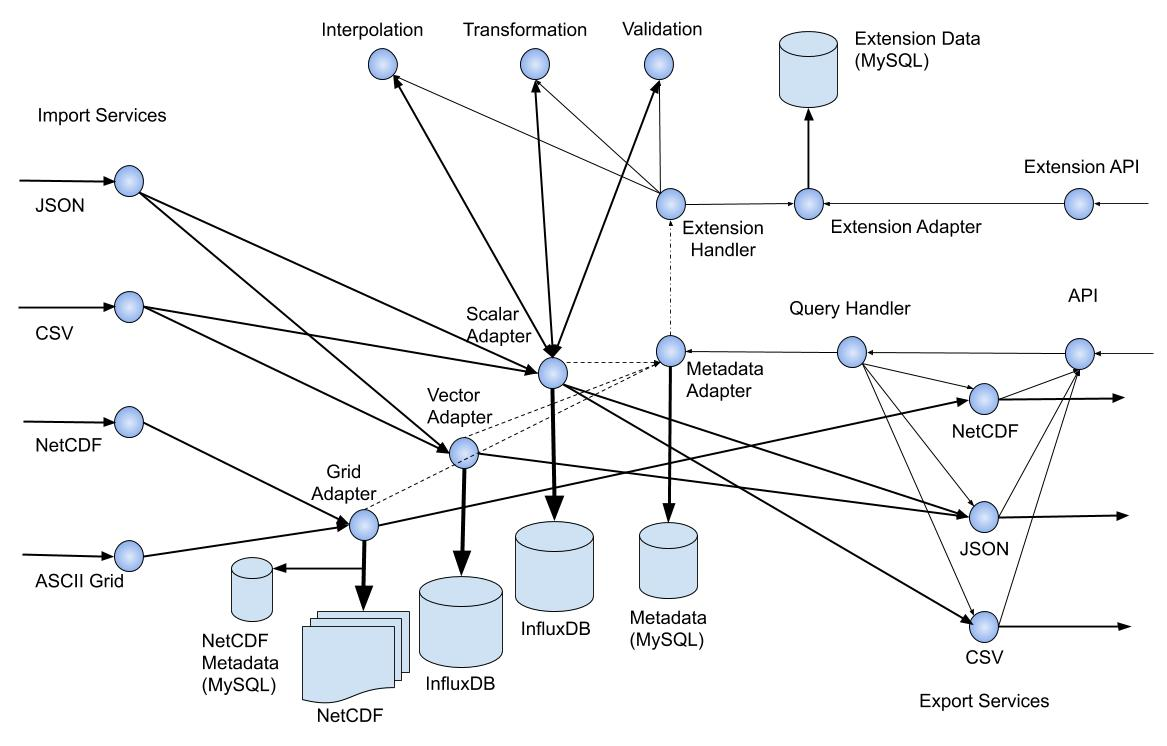
\includegraphics[width=1\textwidth]{method/microservice/microservice_architecture-handle_on_demand-v3.jpg}
    \caption{\acrshort{wdias} architecture for handling requests on demand}
    \label{fi:wdias_micro_on_demand}
\end{figure}
Left side of \cref{fi:wdias_micro_on_demand} shows the import modules of the \acrshort{wdias}, and right side shows the export modules. As it explained section \cref{subse:dumb_pipes}, each import microservice only do specific task of converting and forwarding the request to the correct data adapter module.
For each data type, there is a adapter microservice is running which is optimized to storing such type of data. And the metadata data of the timeseries store using \acrshort{rdbms} which gives more performance over retrieving metadata data. The metadata is cached with In-Memory database to fast access as mentioned in \cref{subse:redis}.
The system generate a unique identifier for each timeseries, and through out the \acrshort{wdias}, other microservice use it to handle data for fast access.

\begin{figure}[htp]
    \centering
    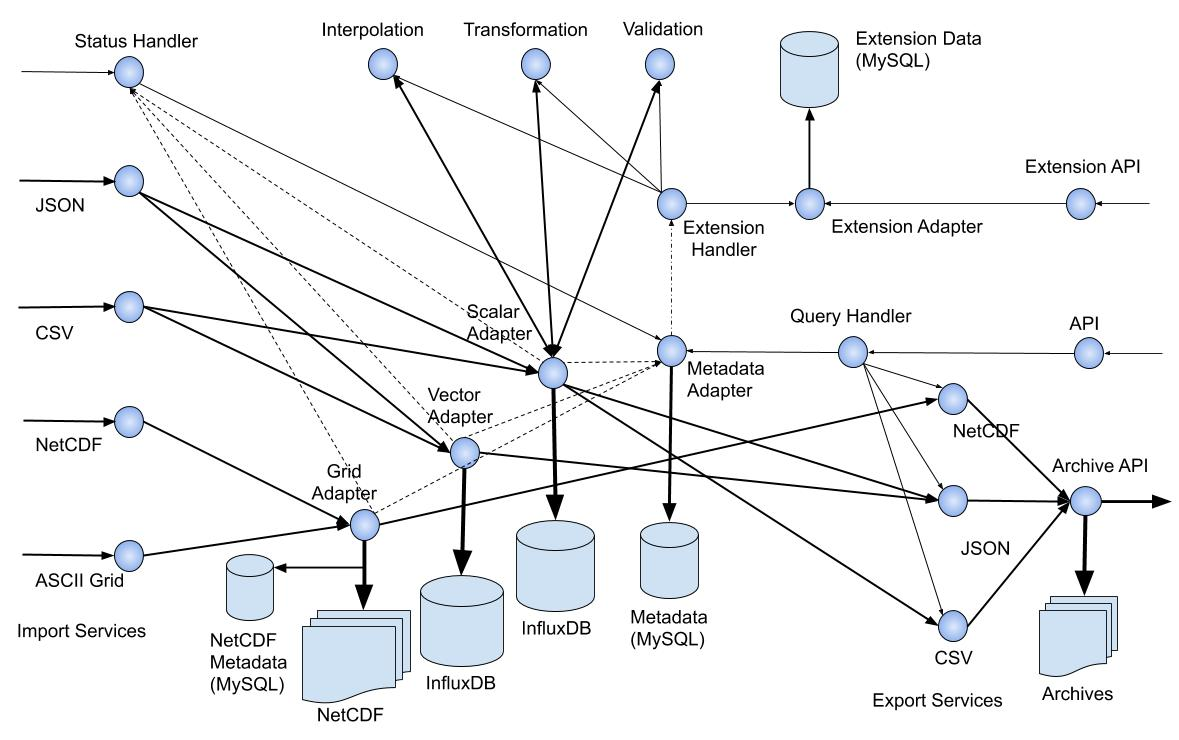
\includegraphics[width=1\textwidth]{method/microservice/microservice_architecture-handle_on_async-v3.jpg}
    \caption{\acrshort{wdias} architecture for handling requests asynchronously.}
    \label{fi:wdias_micro_async}
\end{figure}
Export module microservice follows the same concepts and provide the capability to export the data into required formats of the weather models.
Each adapter follows the concept of database per service as mentioned in the section \cref{subse:database_per_service}. This gives the freedom for \acrshort{wdias} to scale better with \acrshort{k8s}.

As shown in \cref{fi:wdias_micro_on_demand}, when a smaller size request come to the system, it handle on demand and response back. However, as shown in \cref{fi:wdias_micro_async}, when a request with larger size come to the system, it store the data for asynchronously process the data and response with a unique id which can use to verify whether data processed successfully or not. Here is uses the microservice pattern of \cref{subse:sagas} while processing the Grid data. First it store the data and respond back to the user. Then publish an event, and another service listen to those events and process the data and update the system status.

\begin{figure}[htp]
    \centering
    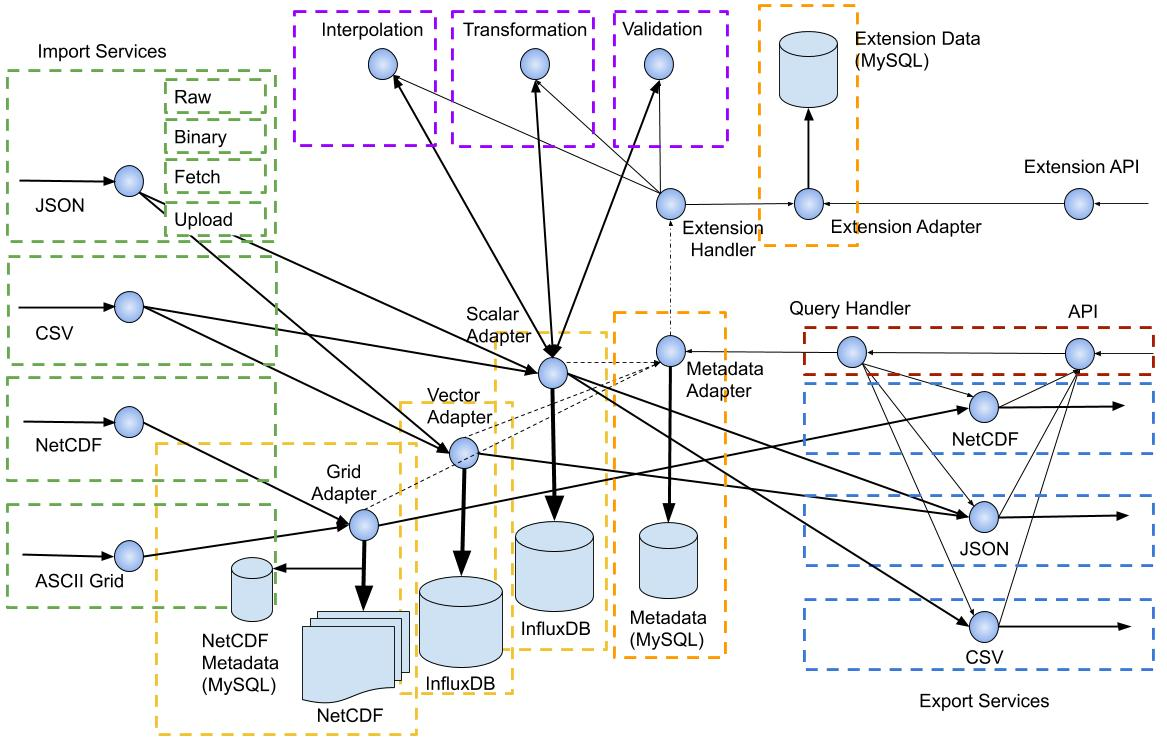
\includegraphics[width=1\textwidth]{method/microservice/separation_microservices-v3.jpg}
    \caption{Separation of \acrshort{wdias} microservices.}
    \label{fi:wdias_micro_separation}
\end{figure}
The \cref{fi:wdias_micro_on_demand} show the clear separation of microservices into the modules of the \acrshort{wdias}. As it shown, each adapter has isolated database, and database is hosted separately for the high performance.
Apart from that, as we further discuss in \cref{se:data_preprocess}, the extension modules are running separately such as Interpolation, Transformation and Validation etc.
The Extension Adapter allow users to register new triggers for the extensions. And extension scheduler triggers the events based on time and extension handler triggers event based on data change.


%%%%%%%%%%%%%%%%%%%%%%%%%%%%%%%%%%%%%%%%%%%%%%%%%%%%%%%%%%%%%%%%%%%%%%%%%%%%%%%%
\subsection{\acrshort{wdias} API}
\label{sebse:wdias_api}
One of the main design consideration in \acrshort{wdias} is the convention of defining the \acrshort{api}. It follows a simple RESTful \acrshort{api}, and allow users to interact with HTTP methods.

\emph{Timeseries} endpoints allow to interact with Metadata Adapter, and those are cache on the Query Handler in order to perform search queries. These are the main endpoints to handle timeseries metadata which defines unique timeseries identifier based on the metadata values. As an example, if it needs to extend the system to store irregular grid data, then it should add another set of location endpoints for storing irregular grid location details.
\begin{itemize}
    \item parameter
    \begin{itemize}
        \item \texttt{GET /parameter} -- Get parameters
        \item \texttt{POST /parameter} -- Create parameter
        \item \texttt{PUT /parameter/id} -- Update parameter
        \item \texttt{DELETE /parameter/id} -- Delete parameter
    \end{itemize}
    \item timeStep
    \begin{itemize}
        \item \texttt{GET /timestep} -- Get TimeSteps
        \item \texttt{POST /timestep} -- Create TimeStep
        \item \texttt{PUT /timestep/id} -- Update TimeStep
        \item \texttt{DELETE /timestep/id} -- Delete TimeStep
    \end{itemize}
\dbc{Format others as above}
    \item location
    \begin{itemize}
        \item \texttt{GET /location} -- Get location points
        \item \texttt{POST /location} -- Create location point
        \item \texttt{PUT /location/id} -- Update location point
        \item \texttt{DELETE /location/id} -- Delete location point
        \item \texttt{GET /location/regular-grid} -- Get regular grids
        \item \texttt{POST /location/regular-grid} -- Create regular grid
        \item \texttt{PUT /location/regular-grid/id} -- Update regular grid
        \item \texttt{DELETE /location/regular-grid/id} -- Delete regular grid
    \end{itemize}
    \item timeseries
    \begin{itemize}
        \item \texttt{GET /timeseries} -- Get timeseries
        \item \texttt{POST /timeseries} -- Create timeseries
        \item \texttt{PUT /timeseries/id} -- Update timeseries
        \item \texttt{DELETE /timeseries/id} -- Delete timeseries
    \end{itemize}
\end{itemize}

\emph{Import} endpoints allow to upload data into the \acrshort{wdias} system.
\begin{itemize}
    \item \texttt{POST /import/json/raw} -- Insert Scalar/Vector timeseries data with JSON body
    \item \texttt{POST /import/csv/raw} -- Insert Scalar/Vector timeseries data in CSV format
    \item \texttt{POST /import/ascii-grid/upload} -- Upload set of ASCII Grid files
    \item \texttt{POST /import/ascii-grid/binary} -- Upload a single ASCII Grid file
\end{itemize}

\emph{Export} endpoints allow to get/download data from the \acrshort{wdias} system.
\begin{itemize}
    \item \texttt{GET /export/json/raw} -- Get Scalar/Vector timeseries data in JSON format
    \item \texttt{GET /export/json/raw?start=2000-01-01\&end=2000-01-03} -- Get Scalar/Vector timeseries data in JSON format for given time period
    \item \texttt{GET /export/netcdf/binary} -- Download Grid data timeseries data in \acrshort{netCDF} format
\end{itemize}

\emph{Extensions} endpoints for configure extensions. These details describes in the \cref{se:data_preprocess}.

As it mentioned above, other than the timeseries metadata which is the core of the data system, other module endpoints start with the module name such as import, export and extension. This allows to add new module system if required.
For import and export modules, then follows by the data format. This provide the flexibility to integrate new data format modules.
Then the endpoint name ends with the data upload/insert data type. Data can upload as a single file with binary or multiple files with upload. Or in the body of the request as raw, and need to send the required headers has mentioned by particular module.
Thus the \acrshort{api} convention of \texttt{\hl{/MODULE/DATA\_FORMAT/DATA\_DATA\_TYPE}} allows users to integrate new import or export modules into the system as well as add new data types.
